\documentclass{article}


%%%%%%%%%%%%%%%% 2020 - 11 - 28 %%%%%%%%%%%%%%%%%%
\usepackage{tikz}
\usetikzlibrary{calc}
\usepackage{pgfplots}
\usepackage{graphicx}
\usepackage{url}

\usepackage{amsmath}
\usepackage{algorithm, algpseudocode}
\renewcommand{\algorithmicrequire}{\textbf{Input:}}
\renewcommand{\algorithmicensure}{\textbf{Output:}}
\algnewcommand{\LeftComment}[1]{\Statex \(\triangleright\) #1}
\usepackage{amsfonts}  % \mathbb{R}
\makeatletter
\newlength{\trianglerightwidth}
\settowidth{\trianglerightwidth}{$\triangleright$~}
\algnewcommand{\LineComment}[1]{\Statex \hskip\ALG@thistlm $\triangleright$ #1}
\algnewcommand{\LineCommentCont}[1]{\Statex \hskip\ALG@thistlm%
  \parbox[t]{\dimexpr\linewidth-\ALG@thistlm}{\hangindent=\trianglerightwidth \hangafter=1 \strut$\triangleright$ #1\strut}}
  
\algnewcommand{\LeftLineCommentCont}[1]{\Statex \hskip\ALG@thistlm%
  \parbox[t]{\dimexpr\linewidth-\ALG@thistlm}{\leftskip=\algorithmicindent \hangindent=\trianglerightwidth \hangafter=1 \strut$\triangleright$ #1\strut}}
  
\usepackage[utf8]{inputenc}
\usepackage[english]{babel}
\usepackage{amsthm}
%%%%%%%%%%%%%%%%%%%%%%%%%%%%%%%%%%%%%%%%%%%%%
\newtheorem{theorem}{Theorem}[section]
\newtheorem{corollary}{Corollary}[theorem]
\newtheorem{lemma}[theorem]{Lemma}
\theoremstyle{definition}
\newtheorem{definition}{Definition}[section]
%%%%%%%%%%%%%%%%%%%%%%%%%%%%%%%%%%%%%%%%%%%%%
\usepackage{minted}


\usepackage{subfig}
\usepackage[export]{adjustbox}% in preamble
%\subfloat[hlof entryi][hsub-captioni]{%
%hfigurei}
%\subfloat[hlot entryi][hsub-captioni]{%
%htablei}

\usepackage{hhline}
\usepackage{makecell, caption, booktabs}
\usepackage{siunitx}

%%The second way (hacky, and depends on an implementation detail of els-cas)
\makeatletter
\def\redefparbox{\def\@parboxrestore{\@arrayparboxrestore\let\\\@normalcr
  \if@minipage\expandafter\@gobbletwo\fi
  \@firstofone{\centering\casscparboxtest}}}
\def\casscparboxtest#1{%
  \ifx\rightskip#1\relax\expandafter\dimen@\else
    \expandafter\@secondoftwo
  \fi\@gobble{#1}}
\makeatother
%%The second way (hacky, and depends on an implementation detail of els-cas)

%%%%%%%%%%%%%%%% 2020 - 11 - 28 %%%%%%%%%%%%%%%%%%



\usepackage{PRIMEarxiv}

\usepackage[utf8]{inputenc} % allow utf-8 input
\usepackage[T1]{fontenc}    % use 8-bit T1 fonts
\usepackage{hyperref}       % hyperlinks
\usepackage{url}            % simple URL typesetting
\usepackage{booktabs}       % professional-quality tables
\usepackage{amsfonts}       % blackboard math symbols
\usepackage{nicefrac}       % compact symbols for 1/2, etc.
\usepackage{microtype}      % microtypography
\usepackage{lipsum}
\usepackage{graphicx}
\graphicspath{{media/}}     % organize your images and other figures under media/ folder

  
%% Title
\title{ on Polynomial Approximation of Activation Function
%%%% Cite as
%%%% Update your official citation here when published 
%\thanks{\textit{\underline{Citation}}: 
%\textbf{Authors. Title. Pages.... DOI:000000/11111.}} 
}


\author{ \href{https://orcid.org/0000-0003-0378-0607}{\includegraphics[scale=0.06]{orcid.pdf}\hspace{1mm}John Chiang} \\
	\texttt{liyue.sun@mail.nankai.edu.cn, john.chiang.smith@gmail.com} \\
}	



\begin{document}
\maketitle


\section{Introduction}
When it comes to applying homomoiphic encryption techqiue to machine learning such as neural network, there is a techquice problem that non-polynomial of activation function  could not be calculated directly in the HE domain. The common way to deal with it is to approximate the activation function using the least-square method, to a polynomial that can be calculated in a HE-based environmental\cite{hadash2018estimate}. Being widely adapted in recent work related to HE\cite{kour2014real}, however, the least-square method maight not be ideal for this task. In this essay, we propose an neat method to approximate the activation function based on the the least squared method. 

Note that the idea of this essay did come to the present author, but we can not garnteen that other researches haven't found it (we should give some time to read the book carefully before trying to develope some own method). In conclude, this is a simple idea that can propaply work for approximating activation function of HE. // %比最小二次乘更容易符合同态加密下的要求    


\section{Least Square Method}
\label{sec:headings}
For a continuous real-value function $f(x)$, a simple version of least square method to approximate $f(x)$ over range $[a, b]$ by a polynomial of a given degree $n$ is to find a polynomial of at most degree $n$, $p_n(x)$, such that  minimise the $$\int_{a}^{b} (f(x) - p_n(x))^2 dx. $$

For approximating a continuous real-value function $f(x)$ over the range $[a, b]$ by a polynomial of a given degree $n$, a simple version of least square method  is to find a polynomial of at most degree $n$, $p_n(x)$, such that  maximise the $$\int_{a}^{b} (f(x) - p_n(x))^2 dx, $$ which has a unique solution (the best approximation). Least square method is such a common method that many softwares implement this method, such as the function  $polyfit( \cdot )$ in Python, Matlab or Octave. For example, only 3 lines of Octave codes is all it needs to fit the activation function $ReLU(x) = max(0, x) $ over the range $[-8, +8]$ by a polynomial of degree 2, resulting in the figure 1:
\begin{minted}
{octave}
x = [-8:0.000001:+8]; 
y = max(0,x);
polyfit(x,y,2) 
\end{minted} 
and we get the polynomial approximation $p_2^{ls}(x) = 0.058594 +  0.500000 \cdot x +  0.750000 \cdot x^2 $


Even through least square method has many advantages, it maight not be the best choice in the sense of a HE-based environment. In the sense of a HE-based environment, we would like to choice a low-degree polynomial due to the expensive HE operations, and also perfer the similiar curve shape between the apprximation polynomial and the function to approximate, even at the cost of losing best appxiromation. Thus, we propose a simple method to conside the gradient(the slope) into the optimal function.  

and its limition in the polynomial approximation of activation function
To minimise the gray area of the is not enough, we perhaps would like a polynomial approximation that has a similiar shape to the activation function, even at the cost of some larger gray area. 

\section{Our Method}
\label{sec:others}

In this section, we present  a simple method based on the least-square method, which  includes  the graduals (shape) of the Polynomial and the activation into  the least-square method, in order to get the desired polynomial approximation that we describled above.
such that  minimise the 
$$\int_{a}^{b} (f(x) - p_n(x))^2 + (f'(x) - p_n'(x))^2 dx. $$

For a toy example, we use this method for the same task above, that is to fit the activation function $ReLU$ over the range $[-8, +8]$ by a polynomial of degree 2 denoted by $p_2^{lg}(x) = c +  b \cdot x +  a \cdot x^2 . $ The question is to minimise the observation loss function 
\begin{equation*}
  \begin{aligned}
F(a, b, c)  = & \int_{-8}^{0} (f(x) - p_2^{lg}(x))^2  dx 
                +\int_{0}^{+8} (f(x) - p_2^{lg}(x))^2  dx
                +\int_{-8}^{0} (f'(x) - p_2^{lg}{'}(x))^2 dx
                +\int_{0}^{+8} (f'(x) - p_2^{lg}{'}(x))^2 dx   \\
            = & [\frac{4}{3}a^2x^3 + (b^2 + 1 - 2b)x + 2a(b - 1)x^2  ]|_{0}^{+8}  + \\
            &[\frac{1}{5}a^2x^5 + \frac{1}{3}b^2x^3 + bcx^2 - \frac{2}{3}bx^3 + c^2x + \frac{1}{3}x^3 - cx^2 + \frac{1}{2}abx^4 - \frac{1}{2}ax^4 + \frac{2}{3}acx^3 ]|_{0}^{+8} + \\
            & [\frac{4}{3}a^2x^3 + b^2x + 2abx^2  ]|_{-8}^0 + \\
            &[\frac{1}{5}a^2x^5 + \frac{1}{3}b^2x^3 + c^2x + bcx^2  + \frac{1}{2}abx^4 + \frac{2}{3}acx^3 ]|_{-8}^{0} + \\
            = & 14472.5\dot{3}a^2 + 357.\dot{3}b^2 + 16c^2  + 682.\dot{6}ac - 357.\dot{3}b + 178.\dot{6} - 64c - 2176a
 \end{aligned}
\end{equation*}
Minimising $F(a,b,c)$ is a problem of unconstrained optimization. To do that, we need to calcuate  the first-order partial derivatives of $F(a,b,c)$ and have them equal to $0$ : 
\begin{equation*}
  \begin{aligned}
F_a(a, b, c) & = 28945.0\dot{6}a +  682.\dot{6}c - 2176 &= 0  \\
F_b(a, b, c) & =  714.\dot{6}b  - 357.\dot{3}  &= 0  \\
F_c(a, b, c) & = 32c  + 682.\dot{6}a - 64 &= 0
 \end{aligned}
\end{equation*}
Solving these equations, we obtain the unique solution and the polynomial approximation, respectly:
\begin{equation*}
  \begin{aligned}
a = 0.0563686709, b = 0.5, c = 0.7974683544, \\
p_n^{lg}(x) = 0.797468 +  0.500000 \cdot x +  0.056369 \cdot x^2 
 \end{aligned}
\end{equation*}
We compare the polynomial generated by least square,  $p_n^{ls}(x)$, with that of our method $p_n^{lg}(x)$. 
\begin{figure}[ht]
\centering

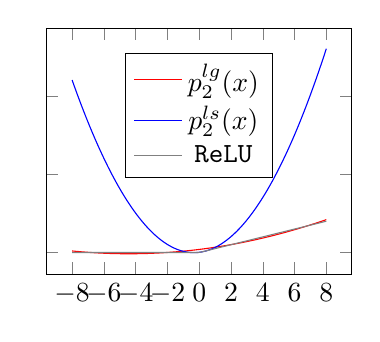
\begin{tikzpicture}[remember picture]
\begin{axis}[ 
%legend pos=south east,
%legend style={at={(0.5,-0.17)},anchor=north,legend cell align=left},
legend style={at={(0.5,+0.9)},anchor=north,},
width=0.45\linewidth, 
xtick={-8, -6, -4, -2, 0, 2,  4, 6, 8 },
yticklabels={}, 
at={(0.66\linewidth,0)},
]
%Below the red parabola is defined
\addplot [
    domain=-8:8, 
    samples=100, 
    color=red,
]
{0.797468 +  0.500000*x +  0.056369*x^2 };
\addlegendentry{$p_2^{lg}(x)$}
%Here the blue parabola is defined
\addplot [
    domain=-8:8, 
    samples=100, 
    color=blue,
    ]
    {0.058594 +  0.500000*x +  0.750000*x^2 };
\addlegendentry{$p_2^{ls}(x)$};
%ReLU
\addplot [
    domain=-8:8, 
    samples=100, 
    color=gray,
    ]
    {max(0, x) };
\addlegendentry{$\texttt{ReLU}$};
\end{axis}
\end{tikzpicture}

\iffalse
\begin{tikzpicture}[overlay, remember picture, scale=.5]
\begin{axis}[ 
hide axis,
%xtick=\empty, ytick=\empty,
width=0.45\linewidth,
%width=3cm,
%height=2.1cm,
%scale only axis,
%xmin=-0.6235,
%xmax=-0.6186,
%xtick={-0.623, -0.621, -0.619},
%ymin=0.1651,
%ymax=0.1655,
%ytick={0.1651, 0.1653, 0.1655},
xshift=2.25cm,yshift=5.75cm,
]
%Below the red parabola is defined
\addplot [
    domain=-2:2, 
    samples=20, 
    color=red,
]
{0.797468 +  0.500000*x +  0.056369*x^2 };
%Here the blue parabola is defined
\addplot [
    domain=-2:2, 
    samples=20, 
    color=blue,
    ]
    {0.058594 +  0.500000*x +  0.750000*x^2 };
%ReLU
\addplot [
    domain=-2:2, 
    samples=20, 
    color=black,
    ]
    {max(0, x) };
\end{axis}
\end{tikzpicture}
\fi

\caption{ Results in the }
\label{fig1}
\end{figure}

\begin{figure}[ht]
\centering

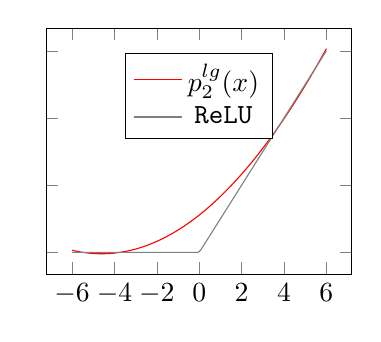
\begin{tikzpicture}[remember picture]
\begin{axis}[ 
%legend pos=south east,
%legend style={at={(0.5,-0.17)},anchor=north,legend cell align=left},
legend style={at={(0.5,+0.9)},anchor=north,},
width=0.45\linewidth, 
xtick={ -6, -4, -2, 0, 2,  4, 6 },
yticklabels={}, 
at={(0.66\linewidth,0)},
]
%Below the red parabola is defined
\addplot [
    domain=-6:6, 
    samples=100, 
    color=red,
]
{1.1110537229 + 0.5*x + 0.054235537*x^2 };
\addlegendentry{$p_2^{lg}(x)$}
%ReLU
\addplot [
    domain=-6:6, 
    samples=100, 
    color=gray,
    ]
    { max(0, x) };
\addlegendentry{$\texttt{ReLU}$};
\end{axis}
\end{tikzpicture}

\caption{ Results in the }
\label{fig2}
\end{figure}
From the figure \ref{fig1}, we can see that our polynomial are much the same as ReLU in the term of shape(slope), and that the least square polynomial doesn't even look like the ReLU funtion.

A more flexiable way to generate teh polynomial approximation is to set add more  parameters to control the weight or propotion of the least square to slope gradial resulting polynomial. To take the $ReLU$  within the domain $[-L, +L]$ as a example, we could optimise the following function:
\begin{equation*}
  \begin{aligned}
F(a, b, c)  =  \lambda_0 \cdot \int_{-L}^{0} (0 - p_2^{lg}(x))^2  dx 
             + \lambda_1 \cdot \int_{0}^{+L} (x - p_2^{lg}(x))^2  dx  \\
             + \lambda_2 \cdot \int_{-L}^{0} (0 - p_2^{lg}{'}(x))^2 dx 
             + \lambda_3 \cdot \int_{0}^{+L} (1 - p_2^{lg}{'}(x))^2 dx , 
 \end{aligned}
\end{equation*}
where $\lambda_0$, $\lambda_1$, $\lambda_2$ and $\lambda_3$ are four real number greater than zero to control the various weight propotion.

Another example is, supposing that we want to find a polynomial to approximate the relu over the domain $[-6, +6]$ such that it fit the ReLU very well at the both ends at the expense of losing some precsion round the center. In this case, we need to minimise the function (we just set $\lambda_0 = \lambda_1 = \lambda_2 = \lambda_3 = 1$ ): 
\begin{equation*}
  \begin{aligned}
F(a, b, c)  =&   \int_{-6}^{-3} (0 - p_2^{lg}(x))^2  dx 
             +  \int_{+3}^{+6} (x - p_2^{lg}(x))^2  dx  
             +  \int_{-6}^{-3} (0 - p_2^{lg}{'}(x))^2 dx 
             +  \int_{+3}^{+6} (1 - p_2^{lg}{'}(x))^2 dx   \\
            =& 3517.2a^2 + 132b^2 + 6c^2  + 54bc + 1917ab + 252ac - 607.5a - 78b - 27c + 12.
 \end{aligned}
\end{equation*}
Solving this  unconstrained optimization, we get the polynomial $p_2^{(1)} = 1.1110537229 + 0.5 \cdot x + 0.054235537 \cdot x^2 $. Figure \ref{fig2} shows that $p_2^{(1)}$ is exactly what polynomial we want. 


\section{Conclusion}
Your conclusion here
Our method to approximate activation function is much flexiable compared to least square method in the sense of ml.
Vouriac setting of parmpaters should result in polynomials of different shapes. 
%Bibliography
\bibliographystyle{unsrt}  
\bibliography{references}  


\end{document}
